\documentclass[a4paper,12pt]{article}

%%% Работа с русским языком
\usepackage{cmap}					% поиск в PDF
\usepackage{mathtext} 				% русские буквы в формулах
\usepackage[T2A]{fontenc}			% кодировка
\usepackage[utf8]{inputenc}			% кодировка исходного текста
\usepackage[english,russian]{babel}	% локализация и переносы
\usepackage{indentfirst}
\frenchspacing



%%% Дополнительная работа с математикой
\usepackage{amsmath,amsfonts,amssymb,amsthm,mathtools} % AMS
\usepackage{icomma} % "Умная" запятая: $0,2$ --- число, $0, 2$ --- перечисление

%% Свои команды
\DeclareMathOperator{\sgn}{\mathop{sgn}}

%% Перенос знаков в формулах (по Львовскому)
\newcommand*{\hm}[1]{#1\nobreak\discretionary{}
{\hbox{$\mathsurround=0pt #1$}}{}}

%%% Работа с картинками
\usepackage{graphicx}  % Для вставки рисунков
\graphicspath{{images/}}  % папка с картинками
\setlength\fboxsep{3pt} % Отступ рамки \fbox{} от рисунка
\setlength\fboxrule{1pt} % Толщина линий рамки \fbox{}
\usepackage{wrapfig} % Обтекание рисунков текстом
\usepackage{minted}

%%% Страница
\usepackage{extsizes} % Возможность сделать 14-й шрифт
\usepackage{geometry} % Простой способ задавать поля
	\geometry{top=25mm}
	\geometry{bottom=35mm}
	\geometry{left=35mm}
	\geometry{right=20mm}

\usepackage{hyperref}
\usepackage[usenames,dvipsnames,svgnames,table,rgb]{xcolor}
\hypersetup{				% Гиперссылки
    unicode=true,           % русские буквы в раздела PDF
    pdftitle={Заголовок},   % Заголовок
    pdfauthor={Автор},      % Автор
    pdfsubject={Тема},      % Тема
    pdfcreator={Создатель}, % Создатель
    pdfproducer={Производитель}, % Производитель
    pdfkeywords={keyword1} {key2} {key3}, % Ключевые слова
    colorlinks=true,       	% false: ссылки в рамках; true: цветные ссылки
    linkcolor=black,          % внутренние ссылки
    citecolor=black,        % на библиографию
    filecolor=magenta,      % на файлы
    urlcolor=blue           % на URL
}

\usepackage{csquotes} % Еще инструменты для ссылок
\author{Карапетян Андрей Варужанович}
\title{Анализатор паролей}
\date{\today}

\begin{document}

\begin{center}
\textbf{Федеральное государственное автономное образовательное учреждение высшего образования \\ "Национальный исследовательский университет \\ "Высшая школа экономики"}\\
\end{center}

\vspace{1em}

\begin{center}
Образовательная программа «Прикладная математика»


\end{center}

\vspace{3em}

\begin{center}
\textbf{ОТЧЕТ}

\textbf{по проектной работе на тему}
\end{center}

\begin{center}
\textbf{<<Анализатор паролей>>}
\end{center}

\vspace{3em}

\begin{flushright}
\textbf{Выполнил студент \\ группы БПМ202}
\vspace{0.6\baselineskip}

Карапетян Андрей Варужанович

\end{flushright}

\vspace{2em}

\begin{flushleft}
\textbf{Руководитель проекта:}
\vspace{1em}

 Белов Александр Владимирович

\vspace{\baselineskip}
\begin{tabular}{lcl}
    \rule{2cm}{0.3pt} & \hspace{1mm} & \rule{2.5cm}{0.3pt}
\end{tabular}

\quad \textit{(оценка)} \hspace{12mm} \textit{(подпись)}

\vspace{1.2\baselineskip}

\rule{5cm}{0.3pt}

\hspace{17mm} \textit{(дата)}
\end{flushleft}

\vspace{\fill}

\begin{center}

Москва

26 мая 2022 г.
\end{center}

\newpage

\tableofcontents

\newpage

\section{Постановка задачи}
Задачей проекта является разработка программного обеспечения, которое способно корректно анализировать введеные пользователем пароли по следующим параметрам:
\begin{enumerate}
\item количество символов; 
\item возможные имена; 
\item возможные фамилии; 
\item даты формата "dd/mm/yyyy"; 
\item возможные клички животных.
\end{enumerate}
Результатом анализа для 2-5 пунктов является вещественное число - вероятность того, что пароль можно идентифицировать как имя, фамилия, дата, кличка животного соответственно.
\newpage

\section{Анализ имеющихся решений}
Исследовав различные интернет-источники, я пришел к выводу, что  поставленная передо мной задача, а также задачи в целом связанные с той или иной оценкой паролей - одной из важнейших компонент защиты множества систем, решается с
помощью методов машинного обучения с учителем, искусственного интеллекта.\\\\ К примеру, авторы сервисов по оценке паролей на сложность, стойкость, время подбора используют слитые базы данных сайтов для того, чтобы оценить, какие сочетания символов в паролях являются наиболее популярными среди обывателей(наверняка знаете про qwertyu; 12345 и тп.). Обучая затем с использованием полученных данных  модели машинного обучения, на основании наличия этих известных сочетаний, а также длины пароля, делается вывод о том насколько сложным является пароль и как долго будет подбирать его машина.\\\\
Решением же конкретно моей задачи может являться обычный перебор. Действительно, загрузив базы данных с именами, фамилиями и кличками, можно просто проверить их наличие в пароле, однако вероятность оценить путем решения задачи таким способом будет невозможно. К тому же перебор будет занимать достаточно большое количество времени. Поэтому для решения задачи все же будут использоваться средства машинного обучения.
\newpage

\section{Синтез алгортима}
Решение задачи можно разделить на несколько шагов:
\begin{enumerate}
\item поиск необходимых баз данных с имена, фамилиями и кличками; 
\item генерация паролей, составление новых баз данных уже с паролями и соответствующими метками; 
\item токенизация и векторизация данных; 
\item обучение классификатора на полученных векторизированных данных;
\item создание GUI;
\end{enumerate}
\subsection{Поиск данных}
Чтобы наш анализатор научился классифицировать имена и тд., необходимо найти в свободных источниках соответствующие базы данных, чтобы после использовать их для составления паролей.
\subsection{Генерация паролей}
Этот шаг необходим, так как мне не удалось в свободном доступе найти базы данных с паролями, включающими в себя только имена, фамилии и тд. из-за чего мне и нужно их составить самому. Для этого будут использованы рандомайзеры, которые будут  составлять случайные пароли, включающие в себя имена, фамилии и прочее.
Также нужно сгенерировать пароли, невключащие в себя необходимые в  условии задачи параметры, чтобы модель успешно могла классифицировать пароли без имен, кличек и тд., а также правильно оценивать вероятности.

\subsection{Токенизация и векторизация}
Для того, чтобы классификатор мог обучиться, необходимо привести наши данные - пароли в числовое представление. Для этого будет использован TF-IDF векторизатор, который оценивает оригинальность сочетаний символов, и считается так:\\
$\text{tf-idf(t,d)} = \text{tf(t,d)} \times \text{ idf(t)}$,\\ где 1 компонента произведения tf(t,d) - количество появлений сочетания символов t в пароле d, 2 компонента произведения\\
$\text{idf}(t) = \log{\frac{1 + n}{1+\text{df}(t)}} + 1$,\\ n - количество паролей, df(t) - количество  паролей, где есть сочетание символов t.\\
Эти сочетания символов также называются токенами, для их получения необходимо токенизация - в нашем случае, просто будем рассматривать отдельные символы пароля как токены. 
\subsection{Обучение классификатора}
Наша задача является задачей классификации - определение наличия в пароле фамилии, имени и тд. 
Классификатор(или модель машинного обучения другими словами) который будет использоваться - логистическая регрессия. Он выбран по причине того, что умеет оценивать вероятности - собственно то, и нужно по условию. Немного про логистическую регрессию.
Функционал ошибки для линейной классификации:\\
$Q(w,X)=1/n*\sum_{i=1}^n \- [y_i (X_i^T w)<0] ,$\\ \text{[]} - индикатор, функция, которую нельзя продифференцировать. По этой причине, градиентный спуск для поиска минимума нельзя использовать. Основная идея - оценить сверху дифференцируемой функцией - к примеру логистической. Тогда получаем такой функционал ошибки, минимум который  путем градиентного спуска можно найти:  \\
$Q(w,X) = \min_{w} \frac{1}{2}w^T w + C \sum_{i=1}^n \log(\exp(- y_i (X_i^T w)) + 1) $,\\ где w - вектор весов признаков, X - матрица объектов, мы ее получили на прошлом шаге, y - вектор правильных ответов, C - коэффициент L2 регуляризации. Таким образом модель сведена к линейной регрессии, полностью аналогична ей.\\
Для задачи обучим 4 классификатора - для получения вероятностей наличия в пароле имен, фамилий, дат и кличек.
\subsection{Создание GUI}
После остается лишь создать удобный интерфейс для программы, а также проверить работоспобность классификаторов на новых данных.
\newpage
\section{Верификация результата}
Проверим полученную программу:\\\\
Введем имя Даша, посмотрим, что выйдет:\\\\
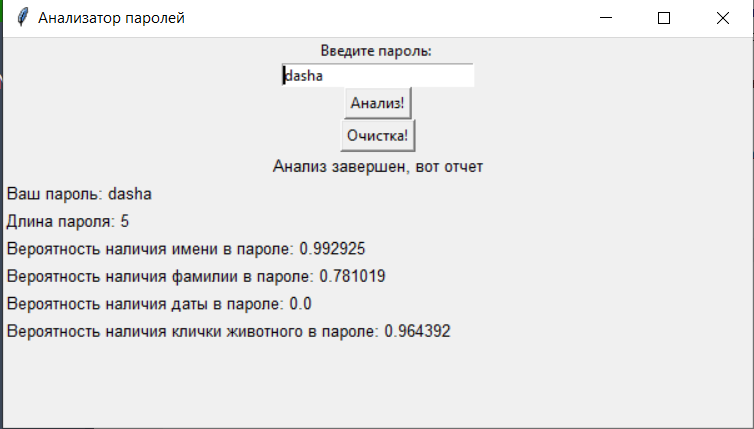
\includegraphics[width=\linewidth]{image1.png}\\\\
Вероятности по имени, кличке и дате оценены хорошо, по фамилии хотелось бы увидеть цифру ниже. Теперь введемм случайный пароль.\\\\
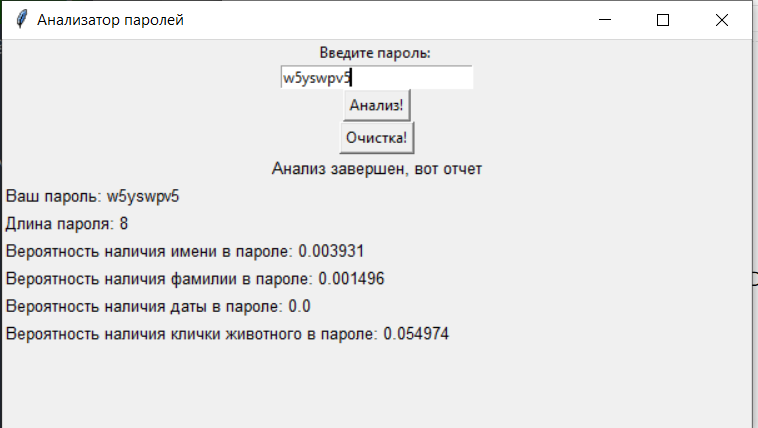
\includegraphics[width=\linewidth]{image2.png}\\\\
Вероятности оценены корректно, теперь введем дату.\\\\
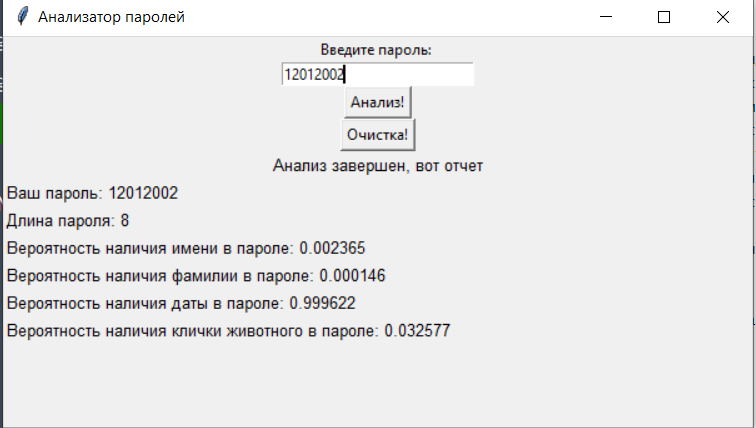
\includegraphics[width=\linewidth]{image3.png}\\\\
Вероятности оценены корректно, теперь введем фамилию.\\\\
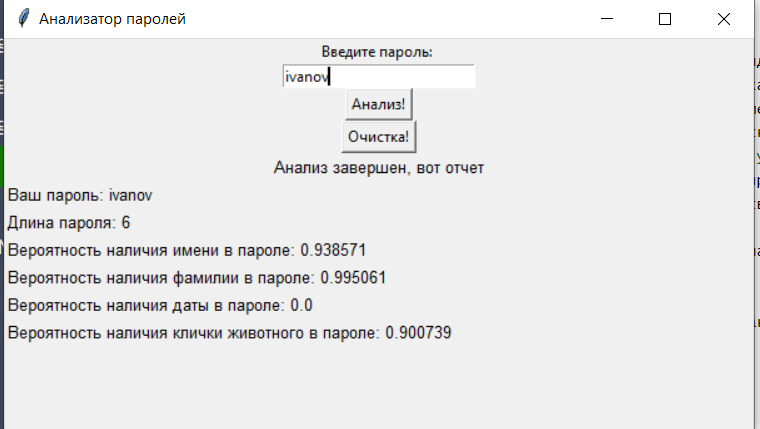
\includegraphics[width=\linewidth]{image4.png}\\\\
Вероятности оценены корректно, теперь введем имя, но добавим цифры.\\\\
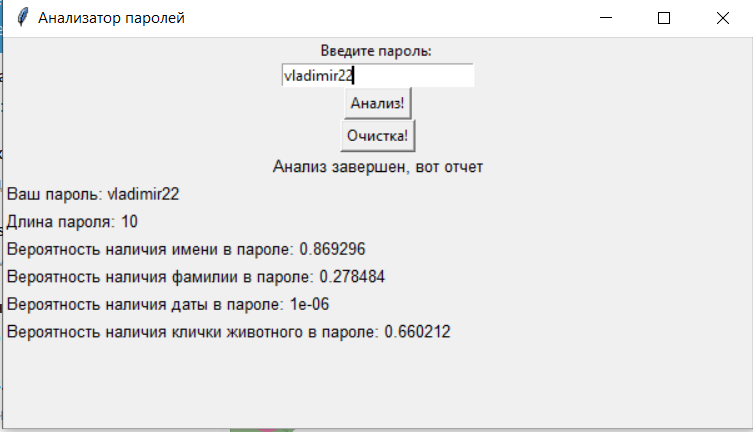
\includegraphics[width=\linewidth]{image5.png}\\\\
На одну цифру больше\\\\.
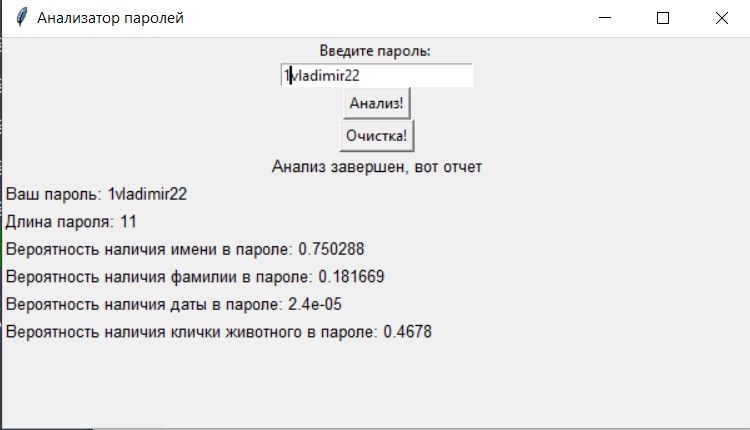
\includegraphics[width=\linewidth]{image6.png}\\\\
Видим, что при добавлении цифры вероятность уменьшается, что корректно. Теперь введем популярный пароль.\\\\
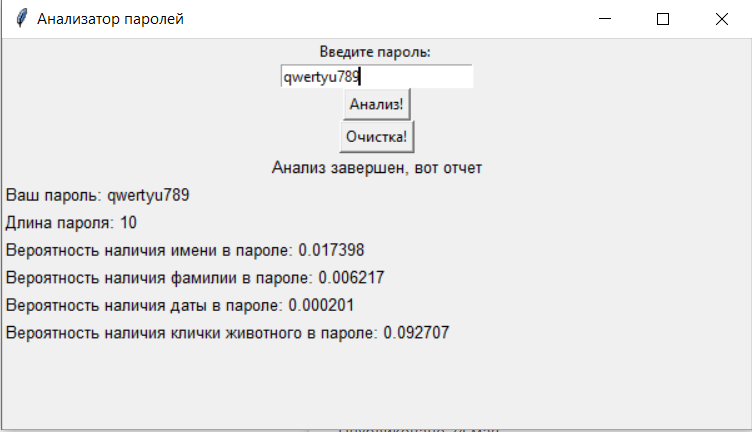
\includegraphics[width=\linewidth]{image7.png}\\\\
Верно. Теперь попробуем кличку пса - bruno.\\\\
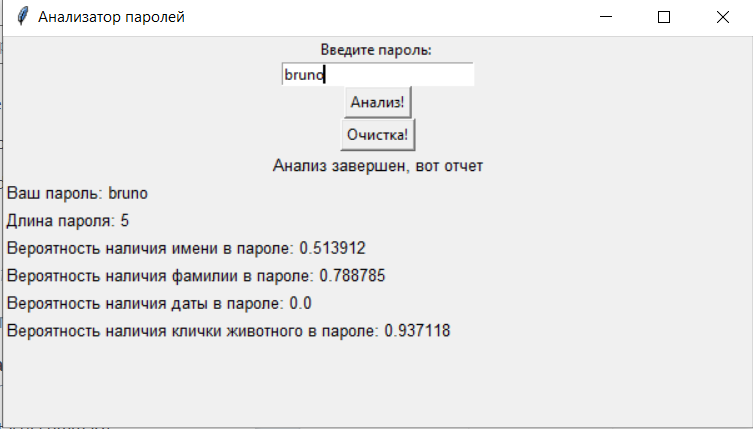
\includegraphics[width=\linewidth]{image8.png}\\\\
Вывод: полнота на высоком уровне(то есть, если есть имя, то оно точно определит, что оно есть), но точность довольно низкая(много неверных прогнозов). Предположение - вина тому, токенизатор, который выдает массив из символов в качестве токенов, из-за чего восприимчивость классификатора резко уменьшается к сочетаниям, укзаывающим на имена, фамилии и тд. , а увеличивается к конкретным символам.
\section{Приложение}
Код программы написан на python 3.10\\
\begin{minted}{python}
import pandas as pd #Импортируем необходимые библиотеки
import string
import random
from sklearn.model_selection import train_test_split
from sklearn.feature_extraction.text import TfidfVectorizer
from sklearn.linear_model import LogisticRegression 
from tkinter import *  
from tkinter import messagebox
import sklearn.utils._typedefs
import sklearn.utils._heap
import sklearn.utils._sorting
import sklearn.utils._vector_sentinel
#базы данных предварительно созданы мной,.
#с помощью генераторов представленных ниже.
characters = list(string.ascii_letters + string.digits)#список разрешенных 
#символов в пароле.

def generate_random_password(name): #генератор паролей для имен, кличек, фамилий.
    length1 = random.randrange(1,4) #символы до имени
    length2 = random.randrange(1,6) #символы после имени
    if len(name)==0:#случай для создания паролей без имен
         length1 = random.randrange(3,9)
         length2 = random.randrange(3,9)
    random.shuffle(characters) 
    password = []
    
    for i in range(length1): #создание пароля в качестве списка
        password.append(random.choice(characters))
    for i in range(len(name)):
        password.append(name[i])
    for i in range(length2):
        password.append(random.choice(characters))

    return "".join(password) #возвращаем в виде строки

def createTokens(f): #Cоздаем токенизатор, он просто возвращаем список символов
    tokens = []
    for i in f:
        tokens.append(i)
    return tokens

def gp(date): #Генератор паролей для дат, работает примерно также, 
#как и для генератор для имен.
    length1 = random.randrange(0,12)
    length2 = random.randrange(0,12)
    random.shuffle(characters)
    password = []
    
    for i in range(length1):
        password.append(random.choice(characters))
    for i in range(len(date)):
        password.append(date[i])
    for i in range(length2):
        password.append(random.choice(characters))

    return "".join(password)

df_names = pd.read_csv('passwords_names') #считываем базу данных 
#с паролями с именами
X_n = df_names['password']#выборка
y_n = df_names['target']#ответы
X_train_n, X_test_n, y_train_n, y_test_n = train_test_split(#перемешиваем 
#объекты в выборке
      X_n, y_n, test_size=0.0000000001, random_state=42)
vectorizer_n = TfidfVectorizer(tokenizer=createTokens)#создаем векторизатор
X_train_n_v = vectorizer_n.fit_transform(X_train_n)#обучаем векторизатор
clf_n = LogisticRegression(max_iter=1000).fit(X_train_n_v, y_train_n)
#обучаем логистическую регрессию

#теперь делаем тоже самое для баз данных с паролями для фамилий, кличек, дат.

df_s = pd.read_csv('passwords_surnames.csv')
X_s = df_s['password']
y_s = df_s['target']
X_train_s, X_test_s, y_train_s, y_test_s = train_test_split(
      X_s, y_s, test_size=0.00001, random_state=42)
vectorizer_s = TfidfVectorizer(tokenizer=createTokens)
X_train_s_v = vectorizer_s.fit_transform(X_train_s)
clf_s = LogisticRegression(max_iter=1000).fit(X_train_s_v, y_train_s)

df_d = pd.read_csv('passwords_dates')
df_d = df_d.fillna('')
X_d = df_d['password']
y_d = df_d['target']
X_train_d, X_test_d, y_train_d, y_test_d = train_test_split(
      X_d, y_d, test_size=0.0000001, random_state=42)
vectorizer_d = TfidfVectorizer(tokenizer=createTokens)
X_train_d_v = vectorizer_d.fit_transform(X_train_d)
clf_d = LogisticRegression(max_iter=1000).fit(X_train_d_v, y_train_d)

df_k = pd.read_csv('passwords_pets')
X_k = df_k['password']
y_k = df_k['target']
X_train_k, X_test_k, y_train_k, y_test_k = train_test_split(
     X_k, y_k, test_size=0.0000001, random_state=42)
vectorizer_k = TfidfVectorizer(tokenizer=createTokens)
X_train_k_v = vectorizer_k.fit_transform(X_train_k)
clf_k = LogisticRegression(max_iter=1000).fit(X_train_k_v, y_train_k)

#создаем интерфейс для программы
def clicked():  
    res = entry.get()
    if len(set(res).intersection(set(characters)))!=len(set(res)):
        messagebox.showinfo('Ошибка!', 'Пароль должен содержать'+ 
        ' только буквы латинского алфавита и цифры!')#ошибка если есть 
        #некорректные символы.
        clear_text()
        return 0
    new = [res]
    new_n_v = vectorizer_n.transform(new)#векторизируем результаты
    new_s_v = vectorizer_s.transform(new)
    new_d_v = vectorizer_d.transform(new)
    new_k_v = vectorizer_k.transform(new)
    predictions_n = clf_n.predict_proba(new_n_v)[0][1]#здесь ищем вероятности 
    #с помощью 4 полученных ранее классификаторов
    predictions_s = clf_s.predict_proba(new_s_v)[0][1]
    predictions_d = clf_d.predict_proba(new_d_v)[0][1]
    predictions_k = clf_k.predict_proba(new_k_v)[0][1]
    analiz[0].pack()
    for i in range(1, 7):
        analiz[i].pack(anchor='w')#выводим отчет
    analiz[0].config(text="Анализ завершен, вот отчет",font=("Arial Bold", 10),)
    analiz[1].config(text="Ваш пароль: "+
    res,font=("Arial Bold", 10))
    analiz[2].config(text="Длина пароля: "+ 
    str(len(res)),font=("Arial Bold", 10))
    analiz[3].config(text="Вероятность наличия имени в пароле: "+
    
    str(round(predictions_n,6)),font=("Arial Bold", 10))
    analiz[4].config(text="Вероятность наличия фамилии в пароле: "+
    
    str(round(predictions_s,6)),font=("Arial Bold", 10))
    analiz[5].config(text="Вероятность наличия даты в пароле: "+
    
    str(round(predictions_d,6)),font=("Arial Bold", 10))
    analiz[6].config(text="Вероятность наличия клички животного в пароле: "+
    
    str(round(predictions_k,6)),font=("Arial Bold", 10))

def clear_text():#функция для кнопки для очистки ввода.
    entry.delete(0, END)
    for i in range(7):
        analiz[i].config(text="")

window = Tk() #окно
window.title("Анализатор паролей")  
window.geometry('600x500')  
lbl = Label(window, text="Введите пароль: ")  
lbl.pack()
entry = Entry(window,width=25)  
entry.pack()
analiz = [Label(window, text="") for i in range(7)]
btn = Button(window, text="Анализ!", command=clicked)#кнопка для анализа 
btn.pack()
btn_clear = Button(window,text="Очистка!", 
command=clear_text)#кнопка для очистки
btn_clear.pack()
window.mainloop()
\end{minted}
\newpage
\section{Источники}
\renewcommand{\refname}{Список источников}
\begin{thebibliography}{99}
\bibitem{names}
База данных по фамилиям и именам:
\href{https://github.com/sorokinpf/russian_names}{https://github.com/sorokinpf/russian_names}
\bibitem{pet names}
База данных по кличкам животных:
\href{https://data.world/anchorage/a9a7-y93v}{https://data.world/anchorage/a9a7-y93v} 
\bibitem{arxiv}
PassGAN: A Deep Learning Approach for Password Guessing \href{https://arxiv.org/abs/1709.00440}{https://arxiv.org/abs/1709.00440} 
\bibitem{Kaspersky}
\href{https://password.kaspersky.com/}{https://password.kaspersky.com/} 
\bibitem{csHSE}
Информация про логистическую регрессию - 
\href{http://wiki.cs.hse.ru/}{http://wiki.cs.hse.ru/} 
\bibitem{sklearn}
Имплементация алгоритмов машинного обучения - 
\href{https://scikit-learn.org/stable/}{https://scikit-learn.org/stable/} 
\end{thebibliography}
\end{document}